\setcounter{figure}{0}   
\setcounter{page}{1}   
\setcounter{section}{0} 
\renewcommand\thefigure{S\arabic{figure}}



{\Huge Supplementary Material}

\section{Other examples}

Final reconstruction of CSC distribution for other samples shown in the text.

\begin{figure}[h!]
    \centering
    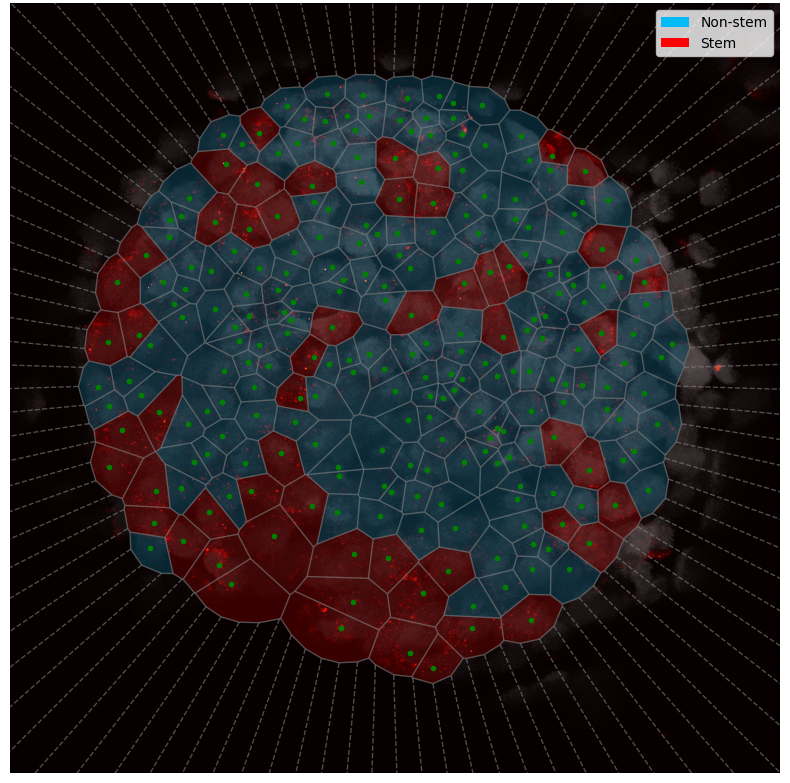
\includegraphics[width=0.8\textwidth]{images/sph1_slice4/nuclei_voronoi_in_sph_only_sox2_clustered_tails_cut_in_sph_with_artificial_boundary_cropped.png}
    \caption{\emph{Voronoi Tessellation overlaid with nuclei and SOX2 fluorescence, colored by stemness (slice 4, \lstinline{Sph1}).} The nuclei fluorescence is shown in a gray scale, whereas the SOX2 fluorescence is shown in a red palette. The centroids of the segmented nuclei are shown as green dots, and the boundaries between the Voronoi regions are plotted with gray lines. Regions have been colored in red (for stem) and blue (for non-stem ones) according to their SOX2 fluorescence content. This layer of cells is below the one seen in Fig. \ref{fig: nuclei voronoi sox2 clustered}. Note how cells that do not belong to the spheroid don't get a region in the tessellation.}
    \label{fig: nuclei voronoi sox2 clustered slice 4}
\end{figure}


\begin{figure}[h!]
    \centering
    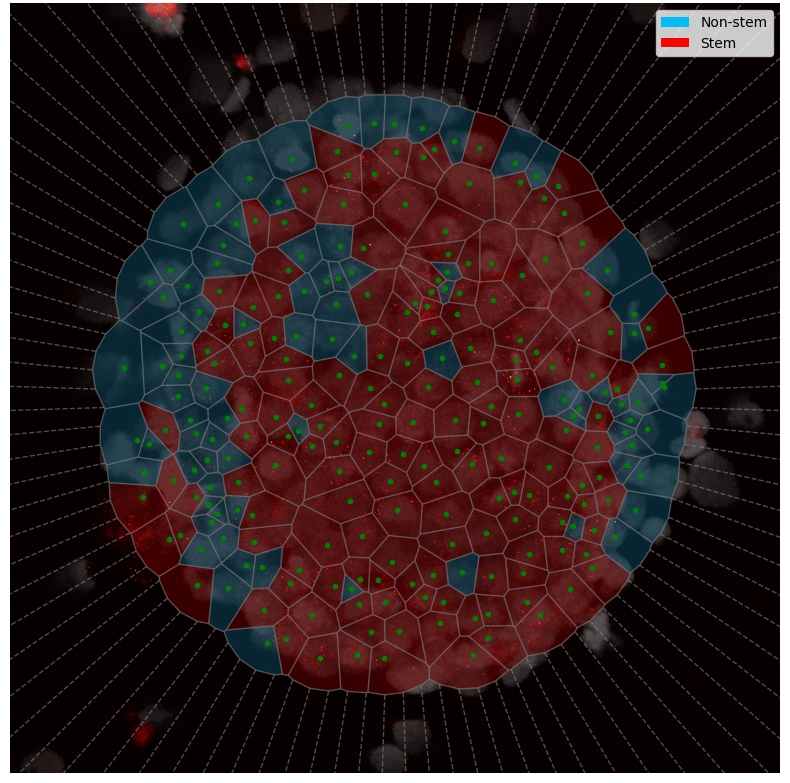
\includegraphics[width=0.8\textwidth]{images/sph3_slice3/nuclei_voronoi_in_sph_only_sox2_clustered_tails_cut_in_sph_with_artificial_boundary_cropped.png}
    \caption{\emph{Voronoi Tessellation overlaid with nuclei and SOX2 fluorescence, colored by stemness (slice 3, \lstinline{Sph3}).} The nuclei fluorescence is shown in a gray scale, whereas the SOX2 fluorescence is shown in a red palette. The centroids of the segmented nuclei are shown as green dots, and the boundaries between the Voronoi regions are plotted with gray lines. Regions have been colored in red (for stem) and blue (for non-stem ones) according to their SOX2 fluorescence content. If the fluorescence surpasses the threshold given by the GMM, the cell is considered a stem one. Regions further away than a certain threshold from the center of the spheroid were excluded from the clustering. Those regions were taken into account for associating the SOX2 to each cell, but their Voronoi cells are not drawn.}
    \label{fig: nuclei voronoi sox2 clustered sph3 slice 3}
\end{figure}




% \section{Delauny triangulation}

% \begin{figure}[h!]
%     \centering
%     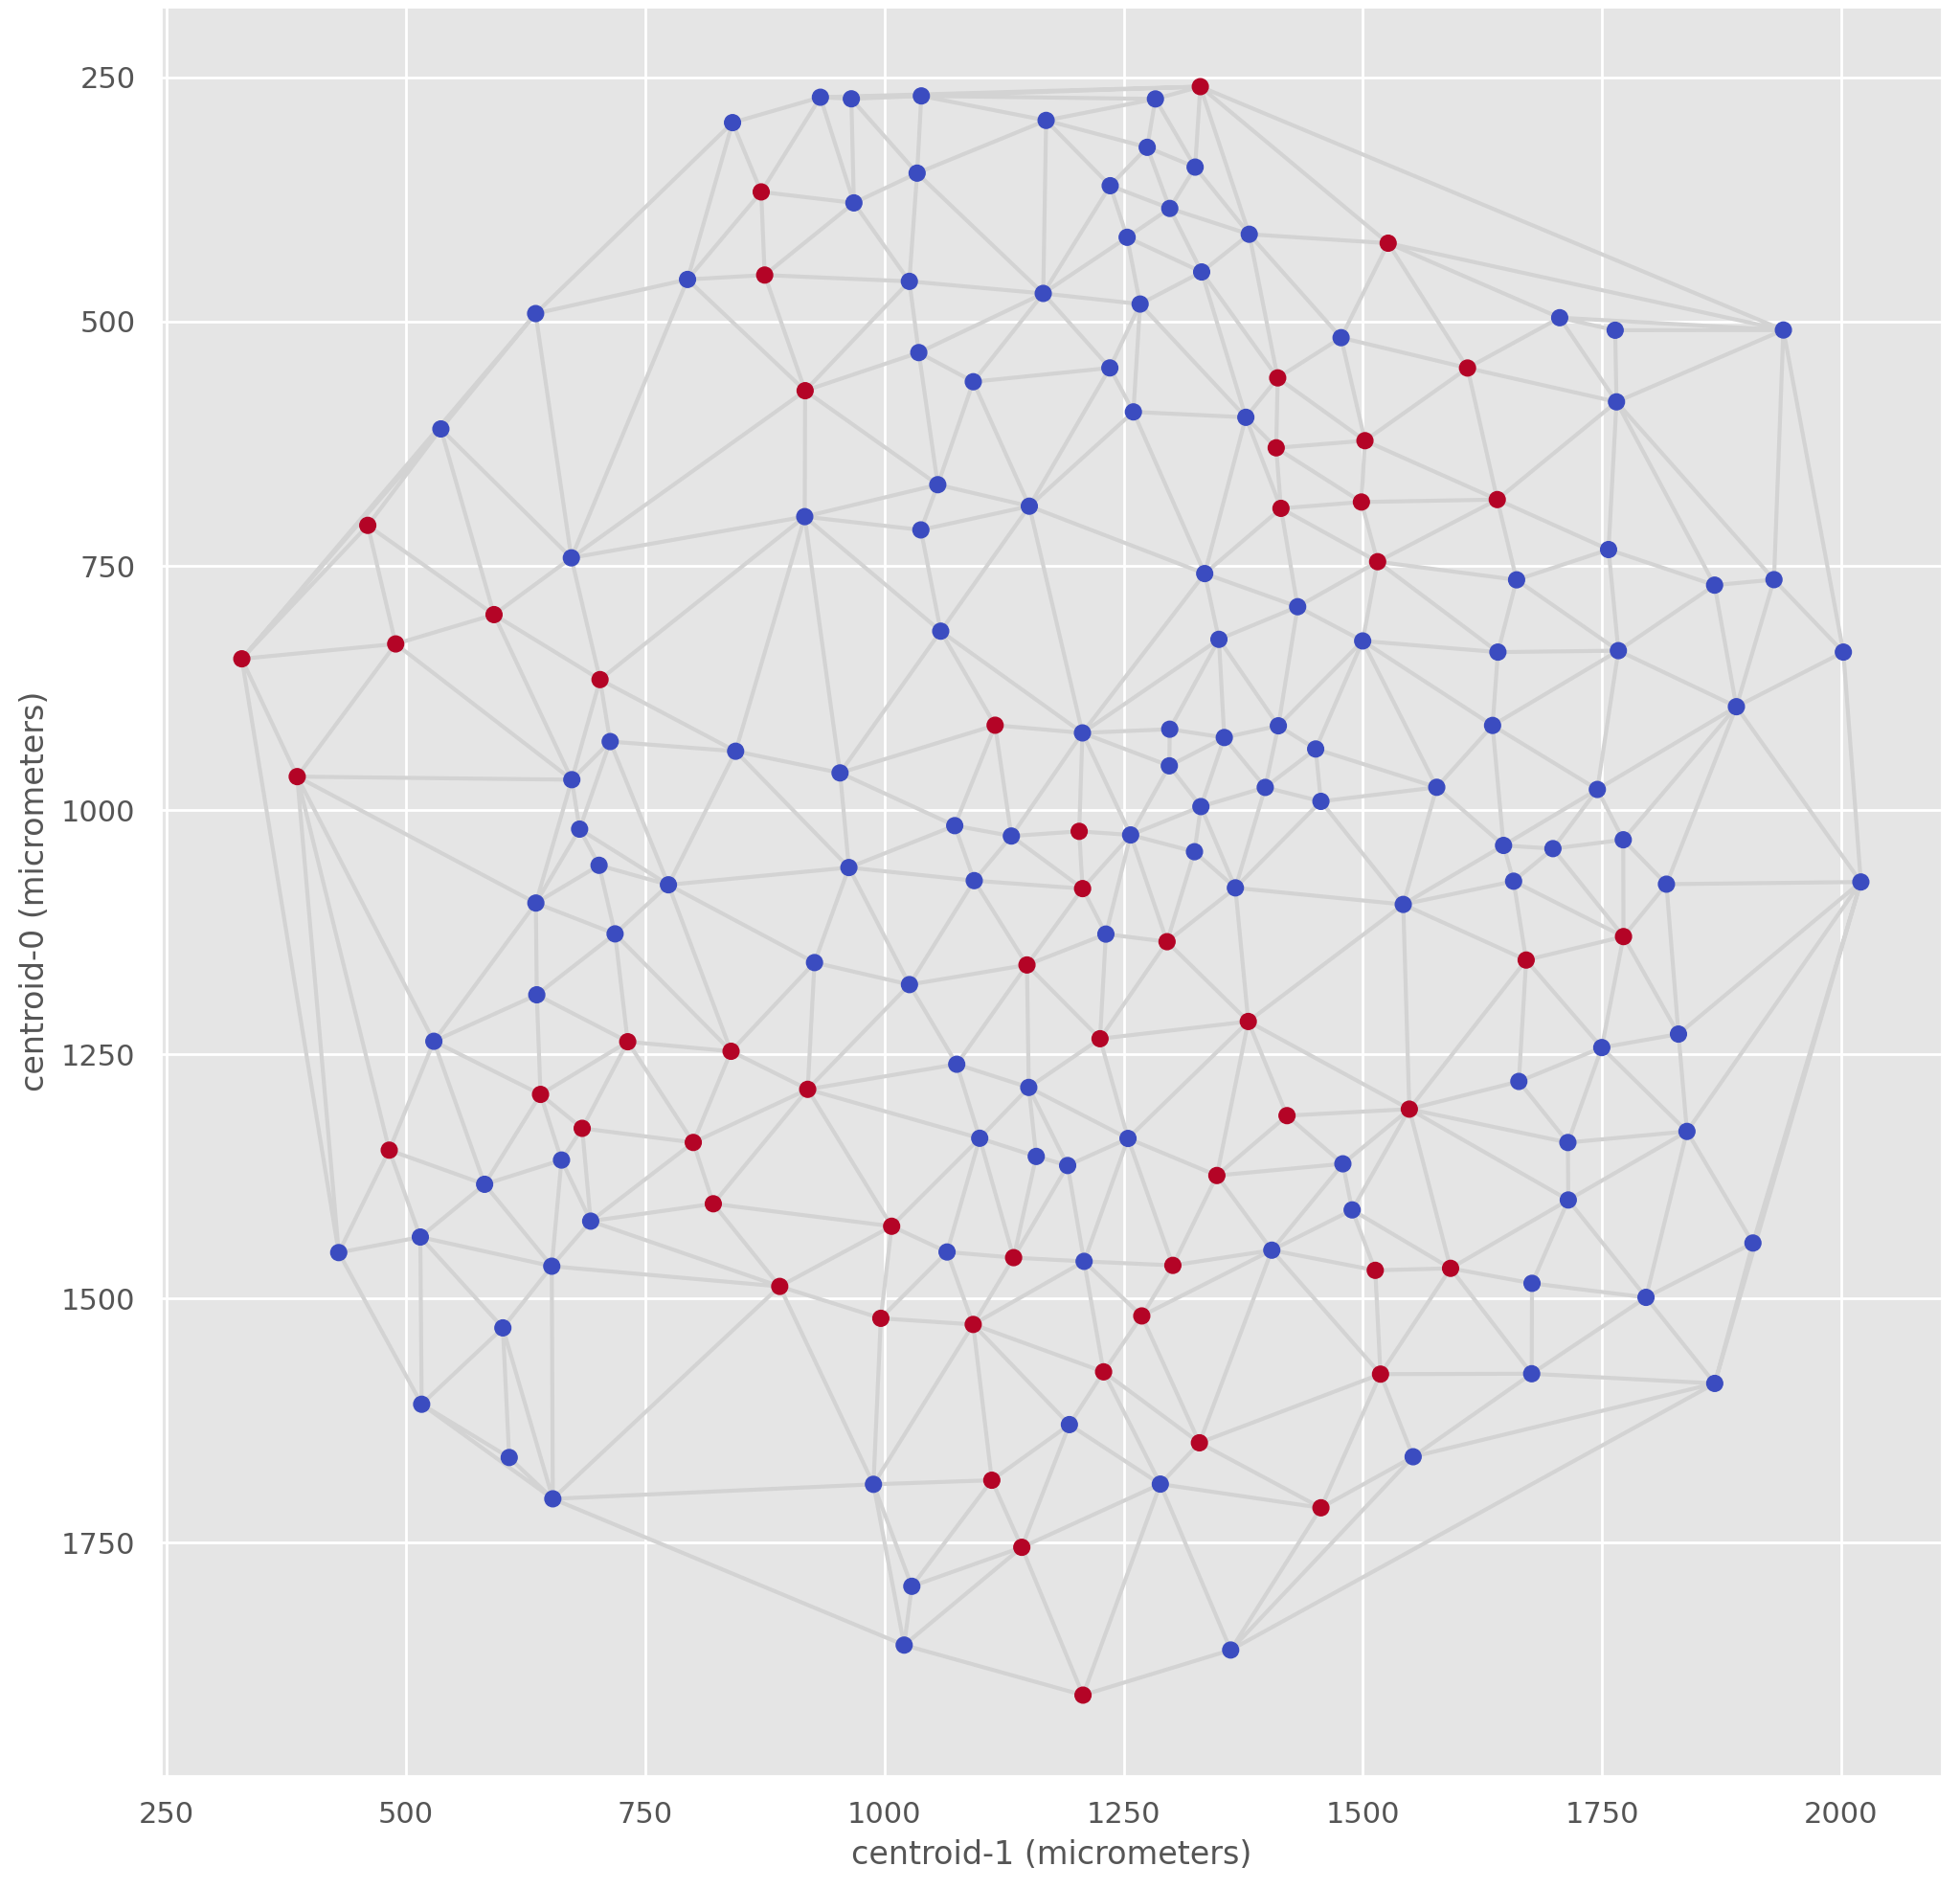
\includegraphics[width=0.9\textwidth]{images/sph1_slice3/delaunay_cropped.png}
%     \caption{\emph{Delaunay triangulation (slice 3, \lstinline{Sph1}).} The network shows Voronoi regions as nodes, and adjacency between regions as edges. Regions corresponding to stem cells are plotted as red dots, while differentiated cells are plotted as blue dots. The axis represent spatial coordinates in the focal plane, measured in micrometers.}
%     \label{fig: Delaunay sph1 slice 3}
% \end{figure}